\chapter{Conclusions and Future Work}
\label{sec:conclusions_and_future_dir}

\fancyhead[LO]{\text{Chapter 7}\quad \text{Conclusions and Future Work}}

This thesis establishes a novel HOPS/AWE algorithm that is particularly well suited to simulating scattering returns for periodic media problems. Our main contribution is that of Theorem $4.6.1$ which guarantees the existence and uniqueness of solutions to a system of partial differential equations which model the interaction of linear waves in periodic layered structures with respect to multiple perturbation parameters. Through the introduction of DNOs and a change of variables based on the TFE methodology, we have shown that solutions to the Helmholtz problem are jointly analytic with respect to both interfacial and frequency perturbations. As a result, our HOPS/AWE algorithm is able to handle a variety of numerical simulations that are physically challenging in both the TE and TM polarization modes. Moreover, our extensive numerical results demonstrate the accuracy, speed, and robustness expected of all HOPS methods.


\section{Future Directions}
\label{Sec: Future Directions}
There are a wide range of improvements to both the HOPS/AWE algorithm and the proof of analyticity for linear waves in periodic layered media. Our main goals for future research are to expand the TFE method through a new proof of convergence, investigate expanding around singularities, evaluate analyticity theorems in multilayered configurations, add new parallel programming functionality, explore alternative methods to recover surface data without Dirichlet--Neumann Operators, and to reduce the execution time of the HOPS algorithm. We now summarize these six research goals and suggest predictions for future research.
\begin{enumerate}[labelsep=0ex,align=left,start=1]
    \item[\textbf{Goal 1-}] ~\textbf{Choice of Parameters: Does the geometry of the perturbation impact how large the size of the perturbation can be? }
    \item[\textbf{Goal 2-}] ~\textbf{Rayleigh Singularities: Can we build a full HOPS algorithm based on points where the Taylor expansion is invalid? }
    \item[\textbf{Goal 3-}] ~\textbf{Multiple Layers: Can we prove analyticity results when the number of layers is greater than three? Do the same theorems hold for ten or one hundred layers?} 
    \item[\textbf{Goal 4-}] ~\textbf{{Parallel Programming}: Can we implement parallel programming techniques so that our HOPS code runs on $N$ processors? }
    \item[\textbf{Goal 5-}] ~\textbf{{Alternatives to DNOs}: Do we need to use DNOs to recover surface data from information stored in the transformed field? Is there an alternative method which preserves the inversion of a single, sparse operator at the interface?   }
    \item[\textbf{Goal 6-}] ~\textbf{Computational Costs: Can we reduce the execution time per time step in our HOPS algorithm?} 
\end{enumerate}

\section{Choice of Parameters}
\label{Sec: Choice of Parameters}
Our HOPS/AWE algorithm is based on two smallness assumptions:
\begin{enumerate}
\item \text{Boundary Perturbation: $g(x)=\varepsilon f(x),$ $\varepsilon\in\mathbb R$, $\varepsilon \ll 1$,}
\vspace{-2mm}
\item \text{Frequency Perturbation: $\omega=(1+\delta)\underline{\omega}=\underline{\omega}+\delta\underline{\omega},$ $\omega\in\mathbb R$, $\delta \ll 1$,} 
\end{enumerate}
with the additional assumption that $f$ is sufficiently smooth ($f\in C^2$ \cite{NichollsReitich99,NichollsReitich03b} or even Lipschitz \cite{hu2005analyticity}). Numerical simulations show that our HOPS/AWE algorithm can handle larger perturbations of $\varepsilon$ (the height/slope) in comparison to $\delta$ (the frequency). With modest test parameters and a period of $d=2\pi$, we are able to perturb the value of $\varepsilon$ (to $\varepsilon=0.1$ or even $\varepsilon=0.2$) and still get reasonable convergence results. At a value around $\varepsilon = 10^{-4}$, our HOPS/AWE algorithm converges to machine precision provided that we sum to high enough Taylor orders.
\vspace{-13mm}
\begin{figure}[H]
    \centering
    \subfloat[\centering Large $\varepsilon$, Small $\delta$ ]{{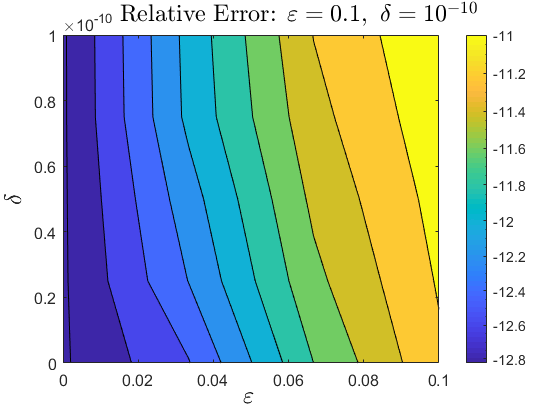
\includegraphics[width=7.6cm]{sections/7_conclusions_and_future_directions/Large_Eps_Small_Delta_2.png} }}%
    %\qquad
    \subfloat[\centering Small $\varepsilon$, Large $\delta$ ]{{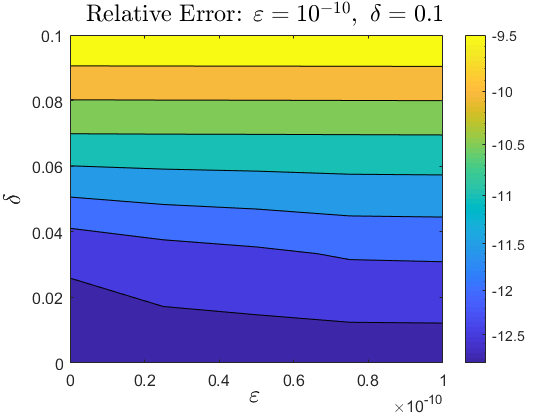
\includegraphics[width=7.6cm]{sections/7_conclusions_and_future_directions/Small_Eps_Large_Delta_2.png} }}%
    \vspace{3 mm}
    \caption{A contour plot of the relative error computed with our HOPS/AWE algorithm by holding $N=M=8$ Taylor orders fixed. In Figure $34\text{(a)}$ we expand up to $\Eps = 0.1$ and $\delta = 10^{-10}$ simultaneously with $N=M=8$ Taylor orders. In Figure $34\text{(b)}$ we expand up to $\Eps = 10^{-10}$ and $\delta = 0.1$ simultaneously with $N=M=8$ Taylor orders.}%
    \label{fig:example}%
\end{figure}
\vspace{-18mm}
Supplementary testing in both the upper and lower layers confirms that our HOPS/AWE algorithm is better suited towards larger $\varepsilon$.
%\begin{flushleft}
\newline
\\
\textbf{Predictions:} Our HOPS/AWE methodology takes advantage of exact enforcement of the \gls{owc} at an artificial boundary in order to truncate the computational domain to one of finite extent. After flattening the surface, the DNOs recover information through the solution stored at the interface. We suspect that this process mitigates large perturbations of the height/slope. By following techniques developed in \cite{NichollsReitich00b,NichollsTaber06,Nicholls16b,NichollsShen08}, we intend to rigorously prove that the TFE method is analytic when $\varepsilon$ is large. Additionally, we are interested in perturbing other physical parameters in the context of layered media problems. These are discussed in the engineering literature \cite{mashayekh2018parameter,mashayekh2018parameter2}.
\section{Rayleigh Singularities}
\label{Sec: Rayleigh Singularities}
A fundamental equation in the HOPS/AWE algorithm is
$$\alpha_p^2 + (\gamma_p^q(\delta))^2 = (k^q)^2,$$
where $k^q$ represents the wavenumber, $q\in\{u,w\}$, and $\alpha=k^q\sin(\theta), \gamma=k^q\cos(\theta),$ are parameters corresponding to refraction/reflection of the incidence angle $\theta$. As shown in $\S 5.4$, a Rayleigh singularity (or Wood's anomaly) occurs when $\ualpha_p^2 = (\uk^q)^2$ for any integer $p\neq 0$. That is, if $\ugamma_p^q(\delta) =0$ for $p\neq 0$ then the Taylor series expansion of $\gamma_p^q(\delta)$ is invalid. In \cite{Nicholls16}, the author investigated changing the Taylor expansion to a Puiseux expansion \cite{basu2007algorithms}:
$$\gamma_p^q(\delta)=\sum_{m=0}^{\infty}\gamma_{p,m}^q\delta^{m+1/2}=\delta^{1/2}\sum_{m=0}^{\infty}\gamma_{p,m}^q\delta^m.$$
However, he found that this approach ran into external difficulties ($\S$6 of \cite{Nicholls16}) simplifying explicit forms of the Dirichlet and Neumann trace operators.
\newline
\\
\textbf{Predictions:} Rayleigh singularities are a central obstruction to the convergence of our HOPS/AWE algorithm. In all of our numerical tests, we select custom frequency ranges which maximize the radius of convergence of our algorithm by expanding away from the singularities (cf. $\S 5.6$). Alternative methods such as Padé summation also fail to be analytic in a neighborhood of a Rayleigh singularity. General perturbation theory provides a variety of known techniques \cite{suslov2005divergent,convfromdiv,Heinz2020,dienes1957taylor,arteca1984summation} for expanding around divergent perturbation series. We suspect that adding these techniques to our HOPS/AWE algorithm will allow us perform a series expansion of $\ugamma_p^q(\delta)$ that does not diverge when $\ugamma_p^q(\delta)=0.$
\section{Multiple Layers}
\label{Sec: Multiple Layers}

In \cite{Nicholls16b}, the author discusses how to apply our HOPS methodology in multilayered configurations. He considers a multilayered material with $M$ (finite) interfaces at 
$$z=a^{(m)}+g^{(m)}(x,y),\quad 1\leq m \leq M,$$
which are $d_x \times d_y$ periodic
$$g^{(m)}(x+d_x,y+d_y)=g^{(m)}(x,y),\quad 1\leq m \leq M,$$
separating $(M+1)$--many layers.
%\vspace{-12mm}
\begin{figure}[H]
    \centering
    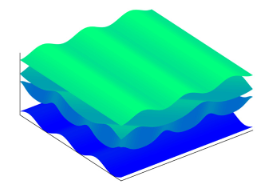
\includegraphics[width=7.6cm]{sections/7_conclusions_and_future_directions/multilayered.png}%
    \vspace{3mm}
    \caption{A five--layer problem configuration with layer interfaces $z = a^{(m)}+g^{(m)}(x).$}%
    \label{fig:example}%
\end{figure}
\vspace{-15mm}
%\begin{flushleft}
A generalization of our analyticity theorems (cf. $\S 4.5$) up to $M$ parameters is included as Theorem~$3.2$ in \cite{Nicholls16b}. For this, we consider quite general systems of linear equations of the form
%\end{flushleft}
\be
\bA(\tEps)\bV(\tEps)=\bR(\tEps),
\ee
where 
\bes
\bA(\tEps)=\sum_{\tn=0}^{\infty}\bA_{\tn}\tEps^{\tn},\quad 
\bR(\tEps) = \sum_{\tn=0}^{\infty}\bR_{\tn}\tEps^{\tn}.
\ees
The tildes represent multi--index notation \cite{Evans10}, in particular
\bes
\tEps := \begin{pmatrix} \Eps_1 \\ \vdots \\ \Eps_M \end{pmatrix},
\quad
\tn := \begin{pmatrix} n_1 \\ \vdots \\ n_M \end{pmatrix},
\ees
and the convention
\bes
\sum_{\tn=0}^{\infty} 
    A_{\tn}\ \tEps^{\tn}
  = \sum_{n_1=0}^{\infty} \cdots \sum_{n_M=0}^{\infty}
    A_{n_1,\ldots,n_M} \Eps_1^{n_1} \cdots \Eps_M^{n_M}.
\ees
As in $\S 4.5$, we seek a solution of the form
\be
\bV(\tEps)=\sum_{\tn=0}^{\infty}\bV_{\tn}\tEps^{\tn},
\ee
and from $(7.1)$ we find at order $\mathcal{O}(\tEps^{\tn})$
\bes
\bA_0\bV_{\tn}= \bR_{\tn} - \left(\sum_{\tl=0}^{\tn}\bA_{\tn-\tl}\bV_{\tl}- \bA_0\bV_{\tn}\right),
\ees
or
\be
\bV_{\tn}= \bA_0^{-1}\left\{\bR_{\tn} - \left(\sum_{\tl=0}^{\tn}\bA_{\tn-\tl}\bV_{\tl}- \bA_0\bV_{\tn}\right)\right\}.
\ee
The above notation represents multi--indices in the form
\bes
\sum_{\tl=0}^{\tn}\bA_{\tn-\tl}\bV_{\tl} = \sum_{\ell_1=0}^{n_1}\cdots \sum_{\ell_M=0}^{n_M}
    \bA_{n_1-\ell_1,\ldots,n_M-\ell_M} \bV_{\ell_1,\ldots,\ell_m},  
\ees
where $\tn=(n_1,\ldots,n_M),$ $\tl=(\ell_1,\ldots,\ell_M),$ and $0=(0,\ldots,0)$ with the convention
\bes
\tn \geq 0 \iff n_1\geq 0,\ldots,n_M\geq 0, \quad\tl \geq 0 \iff \ell_1\geq 0,\ldots,\ell_M\geq 0.
\ees
With these, we can extend our existence theorem (Theorem $4.5.1$) to $M$ parameters.
\begin{theorem}
\label{Thm:AVR}
Given two Banach spaces, $X$ and $Y$, suppose that:
\begin{enumerate}[label={\upshape[\arabic*]}]
\item $\bR_{\tn} \in Y$ for all $\tn \geq 0$,
  and there exist $M$--multi--indexed constants $C_R > 0$, $B_R > 0$,
  \bes
  C_R = \begin{pmatrix} C_{R,1} \\ \vdots \\ C_{R,M} \end{pmatrix},
  \quad
  B_R^{\tn} = \begin{pmatrix} B_{R,1}^{n_1} \\ \vdots \\ 
  B_{R,M}^{n_M} \end{pmatrix},
  \ees
  such that
  \bes
  \Norm{\bR_{\tn}}{Y} \leq C_R B_R^{\tn},
  \ees
\item $\bA_{\tn}: X \rightarrow Y$ for all
  $\tn \geq 0$, and there exist $M$--multi--indexed
  constants $C_A > 0$, $B_A > 0$ such that
  \bes
  \Norm{\bA_{\tn}}{X \rightarrow Y} \leq C_A B_A^{\tn},
  \ees
\item $\bA_0^{-1}: Y \rightarrow X$, and there 
  exists a constant $C_e > 0$ such that
  \bes
  \Norm{\bA_0^{-1}}{Y \rightarrow X} \leq C_e.
  \ees  
\end{enumerate}
Then the equation $(7.1)$ has a unique solution,
\be
\label{Eqn:V:Exp:Multi}
\bV(\tEps) = \sum_{\tn=0}^{\infty} \bV_{\tn} \tEps^{\tn},
\ee
and there exist $M$--multi--indexed constants $C_V > 0$ and $B_V > 0$ such that
\bes
\Norm{\bV_{\tn}}{X} \leq C_V B_V^{\tn},
\ees
for all $\tn \geq 0$ and any
\bes
C_V \geq 2 C_e C_R,
\quad
B_V \geq \max \left\{ B_R, 2 B_A, 2^{M+1} C_e C_A B_A \right\},
\ees
enforced componentwise. This implies that, for any $M$--multi--indexed constant
$0 \leq \tilde{\rho} < 1$, 
$(7.4)$, converges for all $\tEps$ such that
$B \tEps < \tilde{\rho}$, i.e., $\tEps < \tilde{\rho}/B$.
\end{theorem}
\begin{remark}
Our proof strategy is a form of multidimensional induction where given a statement $\bP(n_1, n_2, n_3, ..., n_M)$ for some $M\in \mathbb{N}$, we will show that $\forall n_1, n_2,\ldots, n_M \geq 0$, $\bP(n_1, n_2, n_3, ..., n_M)$ is true by inducting on $n_M$. We will follow the steps outlined below.
\begin{enumerate}
\item Establish $\bP(0,\ldots,n_j,\ldots,0)$ for all $1 \leq j < M$ and $n_1,\ldots,n_j \geq 0.$
\item Given $\bP(n_1,n_2,\ldots,n_j,\ldots,0)$ for all $1 \leq j < M$ and $n_1,\ldots,n_j \geq 0$, establish $\bP(n_1,n_2,\ldots,\bar{n}_j,\ldots,0)$. This can be accomplished through the two steps below.
\begin{enumerate}
    \item Establish $\bP(0,\ldots,\bar{n}_j,\ldots,0)$ for all $\bar{n}_j \geq 0$ (where the hypothesis in $[2]$ gives the required case for $n_j < \bar{n}_j$).
    \item Given  $\bP(n_1,n_2,\ldots,\bar{n}_j,\ldots,0)$ for all $1 \leq j < M$ and $n_1 < \bar{n}_1,  n_2 < \bar{n}_2,\ldots, $ $n_{j-1}  < \bar{n}_{j-1}$ and $\bar{n}_j\geq 0$, establish $\bP(\bar{n}_1,\bar{n}_2,\ldots,\bar{n}_j,\ldots,0)$.
\end{enumerate}
\item Given $\bP(n_1,n_2,\ldots,n_j,n_{j+1},\ldots,0)$ for all $1 \leq j+1 < M$ and $n_1,\ldots,n_{j+1} \geq 0$, establish $\bP(n_1,n_2,\ldots,n_j,\bar{n}_{j+1},\ldots,0)$. This can be accomplished by following the two steps outlined below. 
\begin{enumerate}
    \item Establish $\bP(0,\ldots,\bar{n}_{j+1},\ldots,0)$ for all $\bar{n}_{j+1} \geq 0$ (where the hypothesis in $[3]$ gives the required case for $n_{j+1} < \bar{n}_{j+1}$).
    \item Given  $\bP(n_1,n_2,\ldots,n_j,\bar{n}_{j+1},\ldots,0)$ for all $1 \leq j+1 < M$ and  $n_1 < \bar{n}_1,  n_2 < \bar{n}_2,\ldots, n_{j} < \bar{n}_{j}$ and $\bar{n}_{j+1}\geq 0$, establish $\bP(\bar{n}_1,\bar{n}_2,\ldots,\bar{n}_j,\bar{n}_{j+1}\ldots,0)$.
\end{enumerate}
\item Given $\bP(n_1,n_2,\ldots,n_{M-1},n_M)$ for all $n_1,n_2,\ldots,n_{M-1} \geq 0$ and $n_M < \bar{n}_M$, establish $\bP(n_1,n_2,\ldots,n_{M-1},\bar{n}_M)$. This can be accomplished by the two steps below (the base cases are handled through $[2]$ and $[3]$).
\begin{enumerate}
    \item Establish $\bP(0,\ldots,\bar{n}_{M})$ for $\bar{n}_{M} \geq 0$ (where the hypothesis in $[4]$ handles the required case for  $n_{M} < \bar{n}_{M}$).
    \item Given $\bP(n_1,n_2,\ldots,n_{M-1},\bar{n}_M)$ for all $n_1 < \bar{n}_1, n_2 < \bar{n}_2, \ldots n_{M-1} < \bar{n}_{M-1}$ and $\bar{n}_M \geq 0$, establish $\bP(\bar{n}_1,\bar{n}_2,\ldots,\bar{n}_{M-1},\bar{n}_M)$.
\end{enumerate}
\end{enumerate}

\end{remark}

\begin{proof}{[Theorem 7.4.1]} As with $\tEps$ and $\tn$, we represent $\tilde{\rho}$ by
\bes
\tilde{\rho} := \begin{pmatrix} \rho_1 \\ \vdots \\ \rho_M \end{pmatrix}.
\ees
As before, we will work by induction and consider the general case for finite $M>0$ where we want to establish
\bes
\norm{\bV_{n_1,\ldots,n_M}}_X \leq C_{V,1}\ldots C_{V,M} B_{V,1}^{n_1}\ldots B_{V,M}^{n_M}, \quad \forall n_1,\ldots,n_M\geq 0.
\ees
We prove this via an induction on $n_M$. The base case $n_1,n_2,\ldots, n_{j-1},n_{j+1},\ldots,$ $n_M=0$ and $1 \leq j < M$:
\bes
\norm{\bV_{0,\ldots,n_j,\ldots,0}}_X \leq C_{V,j} B_{V,j}^{n_j}, \quad \forall n_j\geq 0,
\ees
has previously been established by Theorem $4.5.1$ where $\tEps = \Eps_j$ and $\delta=0$. We now assume
\bes
\norm{\bV_{n_1,\ldots,n_j,\ldots,0}}_X \leq  C_{V,1}\ldots C_{V,j}B_{V,1}^{n_1}\ldots B_{V,j}^{n_j}, ~~ \forall n_1,\ldots,n_{j-1}\geq 0,~~ \forall n_j < \bar{n}_j,~~ 1 \leq j < M,
\ees
and seek
\bes
\norm{\bV_{n_1,\ldots,\bar{n}_j,\ldots,0}}_X \leq  C_{V,1}\ldots C_{V,j}B_{V,1}^{n_1}\ldots B_{V,j}^{\bar{n}_j}, ~~ \forall n_1,\ldots,n_{j-1}\geq 0.
\ees
This can be obtained through a chain of $(M-1)$ inductions on $n_1,\ldots,n_j$ where $1 \leq j < M$. For simplicity, we will show what happens in the arbitrary case $n_j$. The base case $n_1,\ldots,n_{j-1}=0$:
\bes
\norm{\bV_{0,\ldots,\bar{n}_j,\ldots,0}}_X \leq  C_{V,j}B_{V,j}^{\bar{n}_j}, \quad \forall \bar{n}_j \geq 0,
\ees
is established by Theorem $4.5.1$ where $\tEps = \Eps_j$ and $\delta=0$. Therefore, we assume
\begin{align*}
\norm{\bV_{n_1,\ldots,\bar{n}_j,\ldots,0}}_X \leq  C_{V,1}\ldots C_{V,j}B_{V,1}^{n_1}\ldots B_{V,j}^{\bar{n}_j},~~\forall n_1  &< \bar{n}_1,\ldots, n_{j-1} < \bar{n}_{j-1},~~ \forall \bar{n}_j \geq 0,\\&~ 1 \leq j < M,
\end{align*}
and seek
\bes
\norm{\bV_{\bar{n}_1,\ldots,\bar{n}_j,\ldots,0}}_X \leq  C_{V,1}\ldots C_{V,j}B_{V,1}^{\bar{n}_1}\ldots B_{V,j}^{\bar{n}_j}.
\ees
Recalling $\tn=(n_1,\ldots,n_j)$ and  $\tl=(\ell_1,\ldots,\ell_j)$, we define
\be
{\sum_{\tl=0}^{\tn}}^{*}\bA_{\tn-\tl}\bV_{\tl} := \sum_{\tl=0}^{\tn}\bA_{\tn-\tl}\bV_{\tl} - \bA_0\bV_{\tn},
\ee
and apply $(7.3),(7.5)$ and the mapping properties of $\bA_{0}^{-1}$ to find
\bes
\norm{\bV_{\bar{n}_1,\ldots,\bar{n}_j,\ldots,0}}_X\leq C_e\left\{\norm{\bR_{\bar{n}_1,\ldots,\bar{n}_j}}_Y + {\sum_{\tl=0}^{\tn}}^{*}\norm{\bA_{\tn-\tl}\bV_{\tl}}_Y\right\}.
\ees
Using the estimates on $\bR_{n_1,\ldots,n_j}$ and $\bA_{n_1,\ldots,n_j}$ (for all $n_1,\ldots,n_j$) and $\bV_{n_1,\ldots,n_j}$ $(n_1 < \bar{n}_1, \ldots, n_j < \bar{n}_j)$ we have
\begin{align*}
\norm{\bV_{\bar{n}_1,\ldots,\bar{n}_j,\ldots,0}}_X &\leq
C_e\Bigg\{C_{R,1}\ldots C_{R,j}B_{R,1}^{\bar{n}_1}\ldots B_{R,j}^{\bar{n}_j} + {\sum_{\tl=0}^{\tn}}^{*}C_{A,1}\ldots C_{A,j}B_{A,1}^{\bar{n}_1-\ell_1}\ldots B_{A,j}^{\bar{n}_j-\ell_j}\\ & \qquad \qquad \qquad \qquad \qquad \qquad \qquad \qquad \times
C_{V,1}\ldots C_{V,j}B_{V,1}^{\ell_1}\ldots B_{V,j}^{\ell_j}\Bigg\} \\& =
C_eC_{R,1}\ldots C_{R,j}B_{R,1}^{\bar{n}_1}\ldots B_{R,j}^{\bar{n}_j} + C_eC_{A,1}\ldots C_{A,j}C_{V,1}\ldots C_{V,j} \\&
~~ \times \left(\frac{B_{A,1}}{B_{V,1}}\right)B_{V,1}^{\bar{n}_1}\cdots \left(\frac{B_{A,j}}{B_{V,j}}\right)B_{V,j}^{\bar{n}_j}{\sum_{\tl=0}^{\tn}}^{*}
\left(\frac{B_{A,1}}{B_{V,1}}\right)B_{V,1}^{\bar{n}_1-\ell_1-1}\cdots \\& ~~ \times
\left(\frac{B_{A,j}}{B_{V,j}}\right)B_{V,j}^{\bar{n}_j-\ell_j-1} \\& \leq
C_eC_{R,1}\ldots C_{R,j}B_{V,1}^{\bar{n}_1}\ldots B_{V,j}^{\bar{n}_j} + C_eC_{A,1}\ldots C_{A,j}C_{V,1}\ldots C_{V,j} \\& ~~ \times
\left(\frac{B_{A,1}}{B_{V,1}}\right)B_{V,1}^{\bar{n}_1}\cdots\left(\frac{B_{A,j}}{B_{V,j}}\right)B_{V,j}^{\bar{n}_j}\left(\frac{1}{1-1/2}\right)^j,
\end{align*}
if $B_{A,k}/B_{V,k} \leq 1/2$, $k=1,\ldots,j$ (implying $B_{V,k} \geq 2B_{A,k}$). We are done if we demand that
\bes
B_{V,k} \geq B_{R,k}, \quad C_eC_{R,k} \leq C_{V,k}/2, \quad 2^jC_eC_{A,k}C_{V,k}(B_{A,k}/B_{V,k}) \leq 
C_{V,k}/2.
\ees
This can be realized if
\bes
C_{V,k} \geq 2C_eC_{R,k}, \quad
B_{V,k} \geq \max\left\{B_{R,k},2B_{A,k},2^{j+1}C_eC_{A,k}B_{A,k}\right\}.
\ees
We then assume
\begin{align*}
\norm{\bV_{n_1,\ldots,n_{j+1},\ldots,0}}_X \leq  C_{V,1}\ldots C_{V,j+1}B_{V,1}^{n_1}\ldots B_{V,j+1}^{n_{j+1}}, ~~ &\forall n_1,\ldots,n_j\geq 0,~~ \forall n_{j+1} < \bar{n}_{j+1},\\&~~ 1 \leq j < M,
\end{align*}
and seek
\bes
\norm{\bV_{n_1,\ldots,\bar{n}_{j+1},\ldots,0}}_X \leq  C_{V,1}\ldots C_{V,j+1}B_{V,1}^{n_1}\ldots B_{V,j+1}^{\bar{n}_{j+1}}, ~~ \forall n_1,\ldots,n_{j}\geq 0.
\ees
As before, this can be obtained through a chain of $M$ inductions on $n_1,\ldots,n_{j+1}$ where $1 \leq j < M$. For simplicity, we will show what happens in the arbitrary case $n_{j+1}$. The base case $n_1,\ldots,n_{j}=0$:
\bes
\norm{\bV_{0,\ldots,\bar{n}_{j+1},\ldots,0}}_X \leq  C_{V,j+1}B_{V,j+1}^{\bar{n}_{j+1}}, \quad \forall \bar{n}_{j+1} \geq 0,
\ees
is established by Theorem $4.5.1$ where $\tEps = \Eps_{j+1}$ and $\delta=0$. Therefore, we assume
\begin{align*}
\norm{\bV_{n_1,\ldots,\bar{n}_{j+1},\ldots,0}}_X \leq  C_{V,1}\ldots C_{V,j+1}B_{V,1}^{n_1}\ldots B_{V,j+1}^{\bar{n}_{j+1}},~~\forall n_1  &< \bar{n}_1,\ldots, n_{j} < \bar{n}_{j},~~ \forall \bar{n}_{j+1} \geq 0,\\&~ 1 \leq j < M,
\end{align*}
and seek
\bes
\norm{\bV_{\bar{n}_1,\ldots,\bar{n}_{j+1},\ldots,0}}_X \leq  C_{V,1}\ldots C_{V,j+1}B_{V,1}^{\bar{n}_1}\ldots B_{V,j+1}^{\bar{n}_{j+1}}.
\ees
In this scenario, $\tn=(n_1,\ldots,n_{j+1})$ and  $\tl=(\ell_1,\ldots,\ell_{j+1}),$ so we apply $(7.3),(7.5)$ and the mapping properties of $\bA_{0}^{-1}$ to find
\bes
\norm{\bV_{\bar{n}_1,\ldots,\bar{n}_{j+1},\ldots,0}}_X\leq C_e\left\{\norm{\bR_{\bar{n}_1,\ldots,\bar{n}_{j+1}}}_Y + {\sum_{\tl=0}^{\tn}}^{*}\norm{\bA_{\tn-\tl}\bV_{\tl}}_Y\right\}.
\ees
Using the estimates on $\bR_{n_1,\ldots,n_{j+1}}$ and $\bA_{n_1,\ldots,n_{j+1}}$ (for all $n_1,\ldots,n_{j+1}$) and $\bV_{n_1,\ldots,n_{j+1}}$ $(n_1 < \bar{n}_1, \ldots, n_{j+1} < \bar{n}_{j+1})$ we have
\begin{align*}
\norm{\bV_{\bar{n}_1,\ldots,\bar{n}_{j+1},\ldots,0}}_X &\leq
C_e\Bigg\{C_{R,1}\ldots C_{R,{j+1}}B_{R,1}^{\bar{n}_1}\ldots B_{R,{j+1}}^{\bar{n}_{j+1}} + {\sum_{\tl=0}^{\tn}}^{*}C_{A,1}\ldots C_{A,{j+1}}B_{A,1}^{\bar{n}_1-\ell_1}\ldots \\ & \qquad \qquad \qquad \qquad \qquad \quad \times
B_{A,{j+1}}^{\bar{n}_{j+1}-\ell_{j+1}}C_{V,1}\ldots C_{V,{j+1}}B_{V,1}^{\ell_1}\ldots B_{V,{j+1}}^{\ell_{j+1}}\Bigg\} \\& =
C_eC_{R,1}\ldots C_{R,{j+1}}B_{R,1}^{\bar{n}_1}\ldots B_{R,{j+1}}^{\bar{n}_{j+1}} + C_eC_{A,1}\ldots C_{A,{j+1}}C_{V,1}\ldots C_{V,{j+1}} \\&
~~ \times \left(\frac{B_{A,1}}{B_{V,1}}\right)B_{V,1}^{\bar{n}_1}\cdots \left(\frac{B_{A,{j+1}}}{B_{V,{j+1}}}\right)B_{V,{j+1}}^{\bar{n}_{j+1}}{\sum_{\tl=0}^{\tn}}^{*}
\left(\frac{B_{A,1}}{B_{V,1}}\right)B_{V,1}^{\bar{n}_1-\ell_1-1}\cdots \\& ~~ \times
\left(\frac{B_{A,{j+1}}}{B_{V,{j+1}}}\right)B_{V,{j+1}}^{\bar{n}_{j+1}-\ell_{j+1}-1} \allowdisplaybreaks\\& \leq
C_eC_{R,1}\ldots C_{R,{j+1}}B_{V,1}^{\bar{n}_1}\ldots B_{V,{j+1}}^{\bar{n}_{j+1}} + C_eC_{A,1}\ldots C_{A,{j+1}}C_{V,1}\ldots C_{V,{j+1}} \\& ~~ \times
\left(\frac{B_{A,1}}{B_{V,1}}\right)B_{V,1}^{\bar{n}_1}\cdots\left(\frac{B_{A,{j+1}}}{B_{V,{j+1}}}\right)B_{V,{j+1}}^{\bar{n}_{j+1}}\left(\frac{1}{1-1/2}\right)^{j+1},
\end{align*}
if $B_{A,t}/B_{V,t} \leq 1/2$, $t=1,\ldots,j+1$ (implying $B_{V,t} \geq 2B_{A,t}$). We are done if we demand that
\bes
B_{V,t} \geq B_{R,t}, \quad C_eC_{R,t} \leq C_{V,t}/2, \quad 2^{j+1}C_eC_{A,t}C_{V,t}(B_{A,t}/B_{V,t}) \leq 
C_{V,t}/2.
\ees
This can be realized if
\bes
C_{V,t} \geq 2C_eC_{R,t}, \quad
B_{V,t} \geq \max\left\{B_{R,t},2B_{A,t},2^{j+2}C_eC_{A,t}B_{A,t}\right\}.
\ees
To complete the general case for finite $M>0$, we assume
\bes
\norm{\bV_{n_1,\ldots,n_M}}_X \leq  C_{V,1}\ldots C_{V,M}B_{V,1}^{n_1}\ldots B_{V,M}^{n_M}, ~~ \forall n_1,\ldots,n_{M-1}\geq 0,~~ \forall n_M < \bar{n}_M,
\ees
and seek
\bes
\norm{\bV_{n_1,\ldots,\bar{n}_M}}_X \leq  C_{V,1}\ldots C_{V,M}B_{V,1}^{n_1}\ldots B_{V,M}^{\bar{n}_M}, ~~ \forall n_1,\ldots,n_{M-1}\geq 0.
\ees
The base case $n_1,n_2,\ldots,n_{M-1}=0$:
\bes
\norm{\bV_{0,\ldots,\bar{n}_M}}_X \leq  C_{V,M}B_{V,M}^{\bar{n}_M}, \quad \forall \bar{n}_M \geq 0,
\ees
has previously been established by Theorem $4.5.1$ where $\tEps = \Eps_M$ and $\delta =0$. Finally, we assume
\begin{align*}
\norm{\bV_{n_1,\ldots,n_{M-1},\bar{n}_M}}_X \leq  C_{V,1}\ldots C_{V,M}B_{V,1}^{n_1}\ldots B_{V,M}^{\bar{n}_M},~~~&\forall n_1  < \bar{n}_1,\ldots, n_{M-1} < \bar{n}_{M-1},\\&~~~~ \forall \bar{n}_M \geq 0,
\end{align*}
and seek
\bes
\norm{\bV_{\bar{n}_1,\ldots,\bar{n}_{M-1},\bar{n}_M}}_X \leq  C_{V,1}\ldots C_{V,M}B_{V,1}^{\bar{n}_1}\ldots B_{V,M}^{\bar{n}_M}.
\ees
In this case, $\tn=(n_1,\ldots,n_M)$ and  $\tl=(\ell_1,\ldots,\ell_M),$ so we apply $(7.3),(7.5)$ and the mapping properties of $\bA_{0}^{-1}$ to find
\bes
\norm{\bV_{\bar{n}_1,\ldots,\bar{n}_M}}_X\leq C_e\left\{\norm{\bR_{\bar{n}_1,\ldots,\bar{n}_M}}_Y + {\sum_{\tl=0}^{\tn}}^{*}\norm{\bA_{\tn-\tl}\bV_{\tl}}_Y\right\}.
\ees
Using the estimates on $\bR_{n_1,\ldots,n_M}$ and $\bA_{n_1,\ldots,n_M}$ (for all $n_1,\ldots,n_M$) and $\bV_{n_1,\ldots,n_M}$ $(n_1 < \bar{n}_1, \ldots, n_M < \bar{n}_M)$ we have
\vspace{-1.5mm}
\begin{align*}
\norm{\bV_{\bar{n}_1,\ldots,\bar{n}_M}}_X &\leq
C_e\Bigg\{C_{R,1}\ldots C_{R,M}B_{R,1}^{\bar{n}_1}\ldots B_{R,M}^{\bar{n}_M} + {\sum_{\tl=0}^{\tn}}^{*}C_{A,1}\ldots C_{A,M}B_{A,1}^{\bar{n}_1-\ell_1}\ldots B_{A,M}^{\bar{n}_M-\ell_M}\\ & \qquad \qquad \qquad \qquad \qquad \qquad \qquad \qquad \times
C_{V,1}\ldots C_{V,M}B_{V,1}^{\ell_1}\ldots B_{V,M}^{\ell_M}\Bigg\} \\& =
C_eC_{R,1}\ldots C_{R,M}B_{R,1}^{\bar{n}_1}\ldots B_{R,M}^{\bar{n}_M} + C_eC_{A,1}\ldots C_{A,M}C_{V,1}\ldots C_{V,M} \\& 
~~ \times \left(\frac{B_{A,1}}{B_{V,1}}\right)B_{V,1}^{\bar{n}_1}\cdots \left(\frac{B_{A,M}}{B_{V,M}}\right)B_{V,M}^{\bar{n}_M}{\sum_{\tl=0}^{\tn}}^{*}
\left(\frac{B_{A,1}}{B_{V,1}}\right)B_{V,1}^{\bar{n}_1-\ell_1-1}\cdots \\& \allowdisplaybreaks~~ \times
\left(\frac{B_{A,M}}{B_{V,M}}\right)B_{V,M}^{\bar{n}_M-\ell_M-1} \\&  \leq
C_eC_{R,1}\ldots C_{R,M}B_{V,1}^{\bar{n}_1}\ldots B_{V,M}^{\bar{n}_M} + C_eC_{A,1}\ldots C_{A,M}C_{V,1}\ldots C_{V,M} \\& ~~ \times
\left(\frac{B_{A,1}}{B_{V,1}}\right)B_{V,1}^{\bar{n}_1}\cdots\left(\frac{B_{A,M}}{B_{V,M}}\right)B_{V,M}^{\bar{n}_M}\left(\frac{1}{1-1/2}\right)^M,
\end{align*}
if $B_{A,i}/B_{V,i} \leq 1/2$, $i=1,\ldots,M$ (implying $B_{V,i} \geq 2B_{A,i}$). We are done if we demand that
\bes
B_{V,i} \geq B_{R,i}, \quad C_eC_{R,i} \leq C_{V,i}/2, \quad 2^MC_eC_{A,i}C_{V,i}(B_{A,i}/B_{V,i}) \leq 
C_{V,i}/2.
\ees
This can be realized if
\bes
C_{V,i} \geq 2C_eC_{R,i}, \quad
B_{V,i} \geq \max\left\{B_{R,i},2B_{A,i},2^{M+1}C_eC_{A,i}B_{A,i}\right\}.
\ees
\end{proof}
Using a similar approach in conjunction with the analysis in Chapters $2$ and $3$, we predict a more general form of Theorems $2.9.2$ and $3.8.1$ exists, which would establish the analyticity of the transformed field with respect to any finite $M > 0$ perturbation parameters.
\vspace{1mm}
\begin{conjecture} 
\label{Conj:u,w:Anal:n:n_m}
Given any integer $s \geq 0$, if $f \in C^{s+2}([0,d])$ and 
$U_{\tilde{n}} \in H^{s+3/2}([0,d])$, $W_{\tilde{n}}\in H^{s+3/2}([0,d])$ such that
\bes
\|U_{\tilde{n}}\|_{H^{s+3/2}} \le K_U B_U^{\tn} , \quad
\|W_{\tilde{n}}\|_{H^{s+3/2}} \le K_W B_W^{\tn} ,
\ees
for constants $K_U, K_W>0$ and $M$--multi--indexed constants $B_U, B_W > 0$, then 
$u_{\tn} \in H^{s+2}([0,d]\times[0,a])$, $w_{\tn}\in H^{s+2}([0,d]\times[-b,0])$ and
\bes
\label{Eqn:u,w:Est:n:n_m}
\|u_{\tn}\|_{H^{s+2}} \le K B^{\tn}, \quad
\|w_{\tn}\|_{H^{s+2}} \le \tilde{K}\tilde{B}^{\tn} ,
\ees
for constants $K,\tilde{K}> 0$ and $M$--multi--indexed constants $B ,\tilde{B}>0$.
\end{conjecture}
\vspace{1mm}
Analogously, a similar procedure would establish a more general form of Theorems $2.10.2$ and $3.9.2$ for the analyticity of the DNOs for any finite $M>0$ perturbation parameters.
\vspace{1mm}
\begin{conjecture} 
\label{Thm:G,J:Anal:n:n_m}
Given any integer $s \geq 0$, if $f \in C^{s+2}([0,d])$ and 
$U_{\tn} \in H^{s+3/2}([0,d])$, $W_{\tn} \in H^{s+3/2}([0,d])$ such that
\bes
\SobNorm{U_{\tn}}{s+3/2} \leq K_U B_U^{\tn}, \quad
\SobNorm{W_{\tn}}{s+3/2} \leq K_W B_W^{\tn},
\ees
for constants $K_U,K_W> 0$ and $M$--multi--indexed constants $B_U, B_W > 0$, then $G_{\tn} \in H^{s+1/2}([0,d])$, $J_{\tn} \in H^{s+1/2}([0,d])$ and
\bes
\label{Eqn:G,J:Est:n:n_m} 
\|G_{\tn}\|_{H^{s+1/2}} \le \tilde{K}\tilde{B}^{\tn}, \quad
\|J_{\tn}\|_{H^{s+1/2}} \le \dbtilde{K} \dbtilde{B}^{\tn},
\ees
for constants $\tilde{K},\dbtilde{K}  > 0$ and $M$--multi--indexed constants $\tilde{B},\dbtilde{B}>0$.
\end{conjecture}
\vspace{1mm}
Upon proving these, one has two key ingredients to the more general version of Theorem $4.6.1$ which establishes the existence and uniqueness of solutions to a system of partial differential equations with respect to $M$ perturbation parameters.
\vspace{1mm}
\begin{conjecture} 
\label{Conj:Main}
Given an integer $s \geq 0$, if $f \in C^{s+2}([0,d])$ then the 
equation $(7.1)$ has a unique solution, $(7.4)$,
and there exist a constant $C > 0$ and $M$--multi--indexed constants $B>0$ such that
\bes
\Norm{\bV_{\tn}}{X^s} \leq C B^{\tn},
\ees
for all $\tn \geq 0$.  This implies that for any $M$--multi--indexed constant
$0 \leq \tilde{\rho} < 1$, $(7.4)$, converges for all $\tEps$ such that
$B \tEps < \tilde{\rho}$, i.e., $\tEps < \tilde{\rho}/B$.
\end{conjecture}
\vspace{1mm}
\textbf{Predictions:} In application oriented fields such as signal processing or sea ice modeling, practitioners work with  multiple frequencies \cite{qiu2005high,bosse1995model,zhao2009multi,blanchard2021high} at short or long wavelengths. Also, as depicted in Figure $35$, the grating surface could have $M$ different layers \cite{imperatore2017perturbation} with distinct values of $g_j(x)=\Eps f_j(x),~j=1,\ldots, M$. A proof of Conjecture $7.4.4$ would enable the freedom to enforce any number of perturbation parameters and obtain an analytic solution. Given the widespread availability of parallel computing resources coupled with additional perturbation parameters associated with elastic media, we believe that future research will force hundreds or even thousands of distinct perturbation parameters, all of which should yield an analytic solution.
\section{Parallel Programming}
\setcounter{section}{5}
\label{Sec: Parallel Programming}

In the case of multiple layered interfaces, we need to compute intermediate DNOs for up to $M$ layers. This will greatly increase the computational cost and execution time of our HOPS/AWE algorithm and we suspect that it will be necessary to introduce parallel programming techniques to offset the computational expense. In the context of the \gls{oe} method, preliminary work \cite{fang2015operator} has been completed in C\texttt{++} to parallelize the computation of Navier's equations \cite{BillinghamKing00,achenbach2012wave}. These techniques can be adapted to the TFE method through the choice of OpenMP \cite{chandra2001parallel}, MPI \cite{snir1998mpi}, or CUDA \cite{sanders2010cuda}.
\newline
\\
\textbf{Predictions:} In two or three dimensions, our HOPS code is robust, efficient and has a runtime less than an hour. A local machine with an Intel Core i$5$ CPU, $8$GB of RAM, and Windows $10$ OS completed almost every simulation in this thesis in less than thirty minutes. However, with ten to one hundred layer configurations, we suspect that many simulations will take on the order of weeks or even months. As a result, it will be necessary to parallelize our Matlab code in a compiled programming language such as C or  C\texttt{++}.

\section{Alternatives to DNOs}
\label{Sec: Alternatives to DNOs}
In Chapter $4$ we wrote our scattering problem as a linear system
\bes
\bA \bV = \bR,
\ees
where, upon expanding $\{\bA,\bV,\bR\}$ in both $\varepsilon$ and $\delta$, we arrived at the flat--interface solution $\bA_{0,0}\bV_{0,0}=\bR_{0,0}$
at order $\mathcal{O}(\varepsilon^0,\delta^0)$. We then saw it was necessary to invert
\bes
\bA_{0,0} = \begin{pmatrix}I & -I\\
-G_{0,0} & -\tau^2J_{0,0}\end{pmatrix}, 
\ees
which features the two DNOs, $G_{0,0}$ and $J_{0,0}$, in order to show the existence and uniqueness of solutions. A primary feature of all HOPS schemes is the inversion of a single, sparse operator $\bA_{0,0}$ through the use of DNOs. However, one may ponder if a different technique could produce a more competitive algorithm that is comparable to our HOPS/AWE algorithm (or even better). Is it absolutely necessary to pass in transformed field data in order to efficiently compute and recover internal information stored at the grating surface?
\\
\newline
\textbf{Predictions:} A primary advantage of our HOPS/AWE scheme is that for every perturbation order, it is only necessary to invert a single sparse operator corresponding to a flat--interface, order--zero approximation. There are a number of competing approaches in general perturbation theory within the context of layered media problems. In regards to electromagnetic wave scattering, Galerkin and boundary element methods are discussed in \cite{escapil2020helmholtz,silva2017quantifying,nakata1990boundary,elschner2012optimization,rathsfeld2006} and a high--order perturbation approach based on boundary integral equations in \cite{dolz2020higher}. High--order schemes for linear waves can be computed using level set methods \cite{sethian1999level} and fast marching methods, as well as other methods involving domain decomposition \cite{el2004comparing,benamou1997domain,larsson1999domain,gong2021convergence,perez2018domain,chan1994domain}. A holistic evaluation of these competing methods could potentially improve our HOPS/AWE algorithm if we found a faster method of inverting linear operators without the use of DNOs.
\section{Computational Complexity}
\label{Sec: Computational Complexity}

One of the fundamental reasons for developing our HOPS/AWE algorithm is its advantageous computational complexity for problems within its domain of applicability.
In comparison with other classical methods, our HOPS/AWE approach has several advantages for computing quantities such as the Reflectivity Map, $R=R(\varepsilon,\delta)$. To demonstrate this we begin
by fixing the problem of computing $R$ for $N_{\Eps}$ many values of 
$\Eps$ and $N_{\delta}$ many values of $\delta$.

In the case of computing the DNOs $G$ and $J$, we recall from $\S 2.11$ and $\S 3.10$ that our HOPS/AWE algorithm requires
$N_x \times N_z$ unknowns at every perturbation order, $(n,m)$, corresponding to
the $N_x$ equally--spaced gridpoints in the lateral direction and the $N_z + 1$ collocation points in the vertical dimension. In $\S 4.5$ we saw that we could write our scattering problem as $\bA(\Eps,\delta) \bV(\Eps,\delta) = \bR(\Eps,\delta)$ where
\bes
    \bA(\Eps,\delta)=\sumn \summ \bA_{n,m}\Eps^n\delta^m, \quad \bR(\Eps,\delta) = \sumn \summ \bR_{n,m}\Eps^{n}\delta^m,
\ees
and
\bes
\label{Eqn:Soln:Two_Param_Append}
\bV(\Eps,\delta) = \sumn \summ \bV_{n,m}\Eps^{n}\delta^m.
\ees
At order $\mathcal{O}(\Eps^n,\delta^m)$ this becomes
\begin{align}
\begin{split}
\bA_{0,0}\bV_{n,m}=&~\bR_{n,m}-\sum_{\ell=0}^{n-1}\bA_{n-\ell,0}\bV_{\ell,m}-\sum_{r=0}^{m-1}\bA_{0,m-r}\bV_{n,r}\\&
-\sum_{\ell=0}^{n-1}\sum_{r=0}^{m-1}\bA_{n-\ell,m-r}\bV_{\ell,r}.
\end{split}
\end{align}
A careful study of $(7.6)$
reveals that the computational complexity of forming the
right--hand side at order $(n,m)$ is
\bes
\BigOh{n m N_x \log(N_x) N_z \log(N_z)}.
\ees
Inverting the operator $\bA_{0,0}$ has complexity $\BigOh{N_x \log(N_x) N_z \log(N_z)}$
so the full cost of computing the $\bV_{n,m}$, 
$\{ 0 \leq n \leq N, 0 \leq m \leq M \}$, is
\bes
\BigOh{N^2 M^2 N_x \log(N_x) N_z \log(N_z)}.
\ees
Once these coefficients are recovered, the cost of summing the series in 
$(\Eps,\delta)$ is minimal, provided it is done in an efficient manner 
(e.g., by Horner's rule \cite{BurdenFaires,AtkinsonHan01}). Our algorithm then 
requires an additional $\BigOh{N_{\Eps} N_{\delta}}$ steps to sum 
over every value of $(\Eps,\delta)$, therefore the full cost of 
computing the Reflectivity Map by our HOPS/AWE method is
\be
\BigOh{N^2 M^2 N_x \log(N_x) N_z \log(N_z) + N_{\Eps} N_{\delta}}.
\ee
In contrast, for a single $(\Eps,\delta)$ pair, a Boundary Integral Method solver with $N_x$ lateral
gridpoints requires time proportional to $\BigOh{N_x^3}$ for Gaussian elimination
to solve the resulting dense system of $N_x$ equations in $N_x$ unknowns
\cite{BurdenFaires,AtkinsonHan01,ColtonKress13}. Applying this 
$N_{\Eps} \times N_{\delta}$ times results in a total computational complexity of
\be
\BigOh{N_x^3 N_{\Eps} N_{\delta}}.
\ee
Thus, once $N_{\Eps}$ and $N_{\delta}$ become large, e.g.,

\bes
N_{\Eps} N_{\delta} > \frac{N^2 M^2 N_x \log(N_x) N_z \log(N_z)}{N_x^3},
\ees
our new algorithm becomes far more efficient. We speculate that the cost of $(7.7)$ could be reduced to
\be
\BigOh{N M \log(NM)N_x \log(N_x) N_z \log(N_z) + N_{\Eps} N_{\delta}},
\ee
provided that we develop a more efficient method of computing the $\bV_{n,m}$, 
$\{ 0 \leq n \leq N, 0 \leq m \leq M \}$, such as reducing the problem space at every step. Alternative approaches to layered media problems have also been proposed by other authors \cite{bai2004reduction,chew2005fast}, including interpolation \cite{atkins2010fast} and Green's function \cite{konno2016fast}.
\newline
\\
\textbf{Predictions:} The combination of implementing parallel programming techniques (through, e.g., OpenMP or CUDA) and reducing the problem space at every step will greatly enhance the speed and fidelity of our HOPS/AWE algorithm. Considering the natural advantage surface methods have over conventional methods, such as finite difference, finite element, and spectral element methods, we expect that our HOPS/AWE algorithm will be among the most competitive available for periodic layered media problems.